\documentclass[12pt]{article}
\usepackage{amsmath}
\usepackage{amsfonts}
\usepackage[paperheight=10in,paperwidth=10in,margin=1in]{geometry}
\usepackage{tikz}
%\usepackage[dvipsames]{xcolor}
\usepackage{tcolorbox}

\usepackage{graphicx}
\graphicspath{{images/}}
\begin{document}
	
\newtcolorbox{mybox}{colback=blue!5!white,colframe=blue}
\begin{tikzpicture}[remember picture,overlay]
\coordinate [below=12cm] (midpoint) at (current page.north);
\node at (current page.north west)
{\begin{tikzpicture}[remember picture,overlay]
	\node[anchor=north west,inner sep=0pt,opacity=0.3] at (0,0) {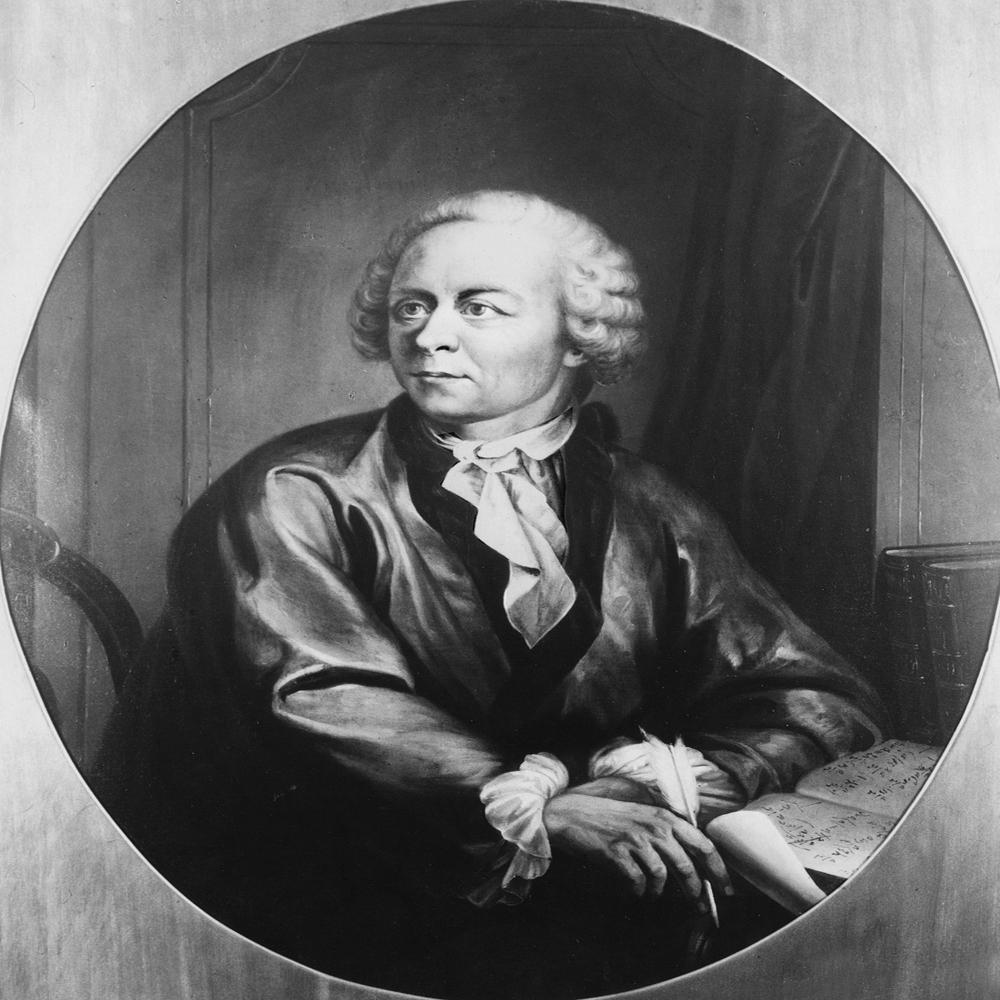
\includegraphics[width=\paperwidth]{euler (1).jpg}}; % Background image
	\end{tikzpicture}};
\end{tikzpicture}
	\begin{center}
		\thispagestyle{empty}
		%\pagecolor{BrickRed}
		%\color{White}
		\color{blue}
		
		\Huge{\textbf{\underline{1000 Followers Special}}}
		
		\vspace*{1cm}
		
		\Huge{\textbf{DM Your Answer!}}
		\vspace*{1cm}
		
		
		\Huge{Find all functions $f: \mathbb{Q}^{+} \rightarrow \mathbb{Q}^{+}$ that satisfy:
			\begin{enumerate}
				\item $f(x+1)=f(x)+1$ $\ ,\ \forall x \in \mathbb{Q}_{+}$
				\item $f(x^2) = f(x)^2$ $\ ,\ \forall x \in \mathbb{Q}_{+}$
			\end{enumerate}}
		
		\vspace{1cm}
		
		\Huge{\textbf{ONLY ELEMENTARY SOLUTIONS WILL BE TAKEN}}
		
		\vspace{1cm}
		
		\Huge{$$\boldsymbol{\sum \limits_{i=0}^{Creative} Math_i = Solving}$$}
		
		\vspace{1cm}
		
		%\begin{mybox}\Huge{\begin{center}\textbf{\textcolor{blue}{Solution $\to$}} \end{center}}\end{mybox}
	\end{center}
\end{document}